% ------- Create Preamble ------------
\documentclass [12pt]{article} 
\usepackage[a4paper]{geometry} 
\usepackage{amsmath, amsthm, amssymb, amsfonts}
 \usepackage{graphicx,epsfig}
\usepackage{booktabs} 
\usepackage{pslatex} 
\usepackage{caption} 
\usepackage{setspace} 
\usepackage{hyperref} 
\usepackage{multicol, multirow}
\usepackage{graphicx,epsfig}
\usepackage{booktabs}
\usepackage{pslatex}
\usepackage{caption}
\usepackage{setspace}
\usepackage{hyperref}
\usepackage{multicol}
\usepackage{textgreek}
\usepackage{pdfpages}
\usepackage{apacite}
\usepackage{float}
\newtheorem{hypothesis}{Hypothesis}
\newtheorem{nullhypothesis}{Null Hypothesis}
\usepackage{tikz}
%---Set up author and title page
\singlespace
\title{The new kids are on the block: incentives for House caucuses to disregard seniority in leadership assignments}
\author{Damon C.\ Roberts\footnote{Ph.D Student,
Department of Political Science, University of Colorado Boulder, UCB 333, Boulder, CO 80309-0333. Damon.Roberts-1@colorado.edu. 
\newline \href{https://github.com/DamonCharlesRoberts/seniority-project}{\textit{Note: }Code and replication data can be found on Github: damoncharlesroberts/seniority-project.}}}}

%set up document
\date{}
\begin{document}
\maketitle
\begin{abstract}

Why might Congressional leaders seek to promote younger and fresher faces in their chambers to leadership positions? In this paper, I provide a theory suggesting that caucus leadership may seek to endorse newer members over those who have been in their respective chamber longer when the benefits provided by the incumbent leader are suspect. Extending this logic, I argue that the promise for partisan teamsmanship is a valuable signal and quite low-cost benefit that less senior members can provide for the cases where incumbent leaders are preforming below the caucus' desires. To be clear, this all relies on the assumption that the increasing professionalization of politicians are correspondingly communicating increased career aspircations.

\end{abstract}

\textbf{Keywords: } Seniority System, House of Representatives, House Leadership, Parties

\newpage
\doublespace
\newpage 
\section*{Introduction}

% TODO Write the Introduction at the end %
The role of the seniority system in the textbook Congress received little attention despite the acute implications of its existence and the eventual institutional and political impacts of its formal removal by Congress in the 1970's \cite{Celler1961}. Since the House of Representatives formally moved away from the seniority system for Committee and other leadership positions, the continued research on the seniority system as an informal institution speaks to the role that it plays as an institution in its own right. The literature is quite well-developed and the scholars interested in studying these sets of questions have quite convincingly settled on the position that following seniority is beneficial to the caucus and to the chamber as a whole.

I argue that the literature of the seniority system needs to better account for situations whereby it is comparatively less beneficial to stick with the seniority system. Building on the existing literature of the seniority system and the motivations that drive legislator behavior in Congress, I argue that there are other incentives that party leaders may pursue that the seniority system cannot provide to the caucus. In my theory, I use the motivations described by \citeA{Fenno1973} as leading factors that actors consider and rely upon as drivers for individual and aggregate behavior. As a result, I hypothesize that Congress remains and institution that tends toward the status quo. In situations where there are clear signals that the challenger can \textit{at least} contribute to maintenance the of caucus' dominance in the chamber and to the career goals of their copartisans. These signals, however, are quite costly. As a result of these costs, situations arise where some of the incumbent leadership are unable to maintain these costs. Starting in this context, my formal model advances my arguments extrapolated from the literature and I conclude that the seniority system is a norm often respected despite individual motives that might suggest otherwise.

\section*{What Seniority Looks Like In The Post-Reform Era}

First, this paper will start out by discussing the existing literature which informs the individual motivations relevant to seniority and leadership assignment. From this discussion, I can then use individual motivations to generalize to what these motivations may look like for the collective - the House caucuses. Once motivations and the assumptions of my theory are established, I can then discuss the likely scenario where the seniority system may be challenged and I discuss the resulting behaviors. 

Central to this theory and the assumptions contained within it is understanding the motivations of individual MC's who are likely working for their own self interest but also it is important to understand the motivations of party leaders who are primarily focused on their caucus and retaining and improving others' status. Before directly addressing the literature on the seniority system, I first am going to explicitly discuss the goals and motivations of members of congress to then move into how a responsible party allows for their members to achieve those to then explore how those motivations may inform the seniority system and how they tie into the existing literature.

\citeA{Mayhew1974} famously claimed that members of Congress seek reelection, above all else. Others have added that MC's also seek to increase their influence by seeking higher position and to make good public policy \cite{Fenno1973}. As a result, institutions are structured in ways to help protect these goals \cite{Mayhew1974}. By implication, MC's push and seek reforms that help them achieve the goal of reelection, by increasing their influence if they want to, and to make good public policy - or at least good for their district. These reforms need not be exclusive to formal rules but they can also be changes to the informal rules which may adjust the norms of the institution. For example, in the late $19^{th}$ century and early $20^{th}$ century, Congress saw a number of changes when "Boss" Reed and "Czar" Cannon shaped the relative power of the Speaker of the House. These adjustment to the norms and rules of the House were meant to centralize control over the House around the speaker. These two MC's when elected to the speaker of the House both sought to discipline those who were not loyal to them but also sought to control the agenda more than any other Speakers had done previously \cite{Cox2005}. Later reforms that helped MC's further achieve benefits was to make a series of reforms in the 1970's.

The House reforms in the 1970's have proven pivotal to shaping the political landscape we observe today. These reforms are also quite influential in scholarly debates about Congress as well. Scholars have long debated whether parties matter in Congress. \citeA{Mayhew1974} proposed a theory where MC's were individualistic and self-interested actors who did not gain much utility from aligning with their party and establishing a solid voting bloc with the other members. Some scholars pitched that parties act as useful voting coalitions that MC's use on some issues and in some contexts; but on some issues, MC's would have to look out for their district and their own interests and vote against their party at a non-trivial rate \cite{Aldrich}. Others who agreed with Mayhew's proposition that parties are not important claimed that pivotal voters in policy gridlock are what mattered; that parties had no power over correcting for gridlock \cite{Krehbiel1991}. 

In the post-reform era, scholars claim that parties have become stronger; largely as a result of the 1970 reforms. \citeA{Rohde1991a} for example claimed that in instances where members of a caucus agree, parties have an impact. That is, parties matter as a voting block to the degree to which there is homogeneity among its members. This Conditional Party Governance theory,  implies that if people agree with their fellow partisans on a particular vote, they are likely to work together as a cohesive unit. Other scholars joined this debate to say that parties matter quite a lot. While parties do not explicitly control and punish those who do not vote a particular way, parties skirt this problem by controlling the available options that are even put before the floor. This Procedural Cartel theory claims that parties seek to maintain their majority status when they have it \cite{Cox2005}. To do so, parties seek to help their members by pushing bills through that matter to their members' constituents and are crucial to seeing the most vulnerable achieve reelection \cite{Cox2005}. While doing this, parties achieve their collective goal - which is to increase the power of its members in Congress, while also assisting individuals realize their personal goals of reelection and an upward career trajectory \cite{Cox2005}. 

The Cartel Theory of parties in Congress provides a compelling starting point for studying the role of seniority. This theory implies that parties are powerful. It implies that members who seek to continue to have party support in their reelection campaigns, their ability to credit claim, their ability to tell their constituents about all of the successes they have representing their interests, need to have some amount of fealty to the party and its leadership. Those who continue to support the collective interest of the party and do their job to push fellow party members' policies within their committee assignment's jurisdiction will be rewarded and will find their job of achieving their individual goals much easier.

These incentives are quite clearly relevant for leadership assignments and seniority. After all, increasing one's relevance and power as a lawmaker begins with increasing one's seniority within the institution. Those who hold subcommittee and coveted committee chairperson titles have more influence in that they have more ability to claim the leadership positions and assignments that they want and may need for their constituents, they have more ability to control the agenda within their policy jurisdictions, and they can increasingly attach their names to other important politicians and issues that increase their district-level and national recognizability. 


While caucus members seek to help one another through the collective good, the current discussion has not yet addressed whether more senior representatives are actually useful to the caucus as a whole. Thankfully, scholars have addressed this question. Overall, it appears that the literature is somewhat skeptical that senior representatives are helpful for helping individual members get reelected and for the party to achieve a maintenance of majority status. As \citeA{Krehbiel1991} argues, seniority is a good thing in Congress - it increases information due to more expertise. That information can then be shared with the general membership and fellow partisans \cite{Krehbiel1991}. By implication, senior members are valuable to the extent that they use and share information to build legislative coalitions to pass effective policy \cite{Taylor2019}. From this, scholars studying the benefits of the seniority system claim that because of this ability to build legislative power are more popular among their constituents in their reelection bids and therefore provide more stability to the caucus leadership. Specifically, \citeA{McKelvey1992} finds that voters do not know or do not care about their representative's relative seniority but instead care about their ability to get things done in congress and whether their representative holds any legislative power to strike bargains. 

This line of work appears somewhat fraught. Scholars studying the origins information in Congress would imply that starting from the point of information as a key factor in support of seniority as a heuristic for assignments is incorrect. A number of scholars have argued that information comes from a number of places in and around Congress \cite{Austen-Smith1993,Hall2006,McCrain2018}. In line with this argument's implications for the seniority system \citeA{Ansolabehere2014} argue that seniority matters very little to voters; voters only care about whether their representative provide observable benefits to the district. Other work not looking at the seniority system support this idea that seniority and its benefits are not what provide stability in membership. For example, more ideologically extreme members tend to be more popular more recently than the moderate ones - those who are likely to have been in Congress longer \cite{Utych2019}. In agreement with \citeA{Ansolabehere2014}, \citeA{Kellermann2009} argue that seniority matters very little. In this instance, \citeA{Kellermann2009} come from the position of the bargaining power you may have to pass legislation rather than the electoral and stability benefits you provide to your caucus. Here, they argue that seniority only impacts the likelihood that you remain on your current committees and the extent to which you face challenges passing legislation in that committee's jurisdiction \cite{Kellermann2009}. That is, those who hold more senior roles on a variety of committees often will face more success at pushing bills through on those policy jurisdictions relative to those who are less senior but do not see any electoral advantages. Seniority, then, is likely to benefit individuals insofar it helps them pursue career goals. For the caucus, having control over the agenda is paramount. With leadership continually pushing the party's agenda forward through strategic assignment, the caucus is more likely to achieve their goal while also helping the caucus' members push good policy for their constituents.

The literature has provided a useful foundation for which to build a theory of seniority's utility upon. The literature indicates a need to assume that parties are relatively strong and that the theory needs to consider a bargain between the party and existing leadership. Parties, it seems, do not benefit in majority status retention from the seniority system. Instead, parties indirectly benefit in this way from the seniority of its members when those senior members effectively provide benefits to their constituents. The path between stability of the caucus' members do not directly come from seniority, but instead they must encourage and not stand in the way of senior members seeking to produce good policy that their constituents will benefit from. The literature also implies that the role of information and the ability to build a coalition is not very strong due to the effectiveness by which parties act as stable coalitions already for those seeking passage of a bill. Individual members who may be less senior, may seek party support and promotion by signaling to the party that they are effective legislators who will be reelected in the future and who aid other members in the caucus in their legislative pursuits. This all is to say that the literature indicates that senior members are not exclusively helpful for the parties. Less senior members must have other attributes and signal these to the caucus. In the next section I provide a simple formal model \footnote{Unfortunately, my knowledge of the method is limited to that of a graduate student who was mediocre in an introductory graduate level game theory seminar.} to articulate my theory in a detailed and comprehensive way. 


\section*{Incentives For Caucus Leadership To Fink On Seniority}

One likely, and perhaps the most interesting, scenario for challengers to arise is when the benefits that the incumbent leader provides are suspect. My theory rests on the assumption that the ability for an individual MC to help their colleagues in the caucuses achieve the goals outlined by \citeA{Fenno1973} is a key metric for others to evaluate their colleagues usefulness. As concluded from the discussion in the previous section, senior members are effective to the degree to which they balance their own career objectives and by providing benefits to their copartisan colleagues. Taking this assumption as true, this would imply that those who hold leadership roles must be among those who provide a number of benefits. Including some nuance in this starting point for my theory, particular benefits may meet a sufficient condition that the caucus needs. Further discussion of the theory will make this point a bit clearer.
  
To begin the discussion, I first outline a number of benefits an individual may bring to the caucus. The first benefit may be that potential leadership may bring electoral advantage to the caucus in a number of ways. The common thread for which they may do this is dependent on a demographic of voter that the party is vying for. For example, both parties seem to be vying for more ideologically extreme candidates in the House of Representatives. Some have argued and provided some empirical evidence indicating that more ideological candidates are more popular among the public, on both sides \cite{Utych2019}. Individuals may also be descriptively aligned with the party or their interests and may be alluring to the party in that way. 

A second benefit that members may provide is policy expertise from prior experience. Parties are not only concerned about reelecting their members. Good public policy is indirectly beneficial to electoral chances of caucus members but they also help build a platform for the party which may help grow the influence of the party across a number of offices at the state level and other levels of the Federal government such as the Senate or the Presidency. If a newly minted representative seeks an assignment and can demonstrate a deep wealth of knowledge for that assignment's jurisdiction when the caucus is concerned with the incumbent's ability to do so, they may prove themselves to be an asset for the party. Moreover, this benefit of expertise increases once one considers how miserly MC's are when it comes to information as discussed in the review of the literature above. Therefore, prior experience with the policy, pre-established networks with bureaucrats or other policy experts, and knowledge about industry and economic reactions to policy implementation, are all benefits that come along with a member who has prior experience and knowledge with a particular policy area. 

These two leading benefits that caucuses may receive from finking on seniority have some powerful impacts on the decision making of assignments. Crucially important is that this all depends on whether the incumbent leader is considered to be doing their job or not. Regardless of whether they are facing a challenger or are leaving the position, the caucus will evaluate challengers based on the comparative benefits to the incumbent that less senior members may provide. To be explicit about the motivations for incumbent position holders and the caucus equations \ref{eq:1} and \ref{eq:2} provides a simple demonstration of this in mathematical notation. 

Equation \ref{eq:1} depicts the argument that the caucus wants to maximize the benefits they receive from those in leadership positions. In equation \ref{eq:1} $C$ represents the caucus and $\beta$ is the benefits that $C$ wants from either the incumbent, $i$, denoted as $\beta_i$, or from less senior members, $m$, denoted as $\beta_m$. The caucus wants chairpersons who favorably examine the proposed legislation from their colleagues - they want them to be team players. They want the influential leaders of the caucus to be effective at expressing the party's agenda as well as being a representative and well-regarded member of that party for the caucus member's respective bases of electoral support. That is, for the caucus, their singular focus is to maximizes the benefits coming from the party - be electorally viable, efficiently pass legislation critical to the party's platforms and goals, and to have members who play well with the public. 

\begin{equation} \label{eq:1}
	C_\beta = \DeclareMathOperator{argMax}{(\beta_i)}
\end{equation}


Another assumption of the model, captured by equation \ref{eq:2}, is that the incumbent, $i$ seeks the opposite scenario. They seek to provide just enough benefits, $\beta$, to hold the assignments they have. As concluded from the literature in the previous section of the paper, members have a number of expectations that they have to balance at once. In practicality, this means that members seek ways to subsidize their work by using lobbyists, for example, to help write legislation \cite{McCrain2018}. With the need to keep up with the desires of the caucus and their constituent, these members seek to find ways to be most efficient - to minimize the benefits they provide to the caucus and to their constituents while also achieving their career goals \cite<see>{Fenno1973,Mayhew1974}. 

\begin{equation} \label{eq:2}
	i_\beta = \DeclareMathOperator{argMin}{(\beta_i)}
\end{equation}

\begin{equation} \label{eq:3}
	\prod \DeclareMathOperator{argMax}{(\beta_i)} > \prod \DeclareMathOperator{argMin}{\beta_i}	
	\equiv
	C_\beta > i_\beta
\end{equation}

\begin{equation} \label{eq:4}
	\prod \DeclareMathOperator{argMax}{(\beta_i)} \approx \prod \DeclareMathOperator{argMin}{\beta_i}
	\equiv
	C_\beta \approx i_\beta
\end{equation}

\begin{equation} \label{eq:5}
	m_\beta = \DeclareMathOperator{argMin}{(\beta)}
\end{equation} 

\begin{equation} \label{eq:6}
	\prod\DeclareMathOperator{argMax}{(\beta_m)} \approx \prod\DeclareMathOperator{argMin}{(\beta_m)}
	\equiv
	C_\beta \approx m_\beta
\end{equation}




With these competing motivations, we are in a world of fragile equilibria. If there is any imbalance in equation \ref{eq:3}, it kicks off a series of events. Figure \ref{fig:tree} presents such a world. Figure \ref{fig:tree} demonstrates a very simple formal model including the payoffs included for both the caucus ($C$) and members ($m$) that could be feasibly selected to replace incumbents ($i$). The figure still includes the considerations from equations \ref{eq:1} and \ref{eq:2}. The remainder of the section is detailing how this formal model informs my theory.


\begin{figure}
% Node styles
\begin{center}

\tikzset{
% Two node styles for game trees: solid and hollow
solid node/.style={circle,draw,inner sep=1.5,fill=black},
hollow node/.style={circle,draw,inner sep=1.5,fill=white}

}

\begin{tikzpicture}[scale=1.5,font=\footnotesize] 

% Specify spacing for each level of the tree
\tikzstyle{level 1}=[level distance=15mm,sibling distance=15mm]
\tikzstyle{level 2}=[level distance=10mm,sibling distance=35mm]
\tikzstyle{level 3}=[level distance=10mm,sibling distance=13mm]
\tikzstyle{level 4}=[level distance=12mm,sibling distance=13mm]
\tikzstyle{level 5}=[level distance=10mm,sibling distance=15mm]
% The Tree
\node(0)[solid node,label=above:{$N_1$}]{} 
child{node(1)[solid node, white]{}
}
child{[white] node(2)[solid node, yshift=-35]{$C$} %note that you need to adjust the yshift if you change the sibling distance
child{[black] node(4)[solid node, label=above:{$N_2$}]
child{node(5)[solid node,white]{}}
child{[white] node(6)[solid node, yshift=-30]{$C$} 
child{[black] node(8)[solid node, label=above:{$m$}]{}
child{[black] node(9)[solid node, label=below:{($1-\delta_c, 1-\delta_m + \beta_a$)}]{} edge from parent node[left]{$a$}}
child{[black] node(9)[solid node, label=below:{($1-\delta,1$)}]{} edge from parent node[left]{$\tilde a$}}
	edge from parent node[left]{$p$}
	}
child{[black] node(8)[solid node, label=below:{$(1 -(1-\beta_i),1)$}]{} edge from parent node[left]{$\tilde p$}}
edge from parent node[black,xshift=0,yshift=-20]{$\beta_m\epsilon[0,1]$}
}
child{node(7)[solid node,white]{}
}
edge from parent node[left]{$S$}
}
child{[black] node(4)[solid node, label=below:{$(1, 1)$}]{}
edge from parent node[right]{$\tilde S$}
}
 edge from parent node[black, xshift=0,yshift=-42]{$\beta_i\epsilon[0,1]$} %note that you need to adjust the yshift if you change the level distance
}
child{node(3)[solid node, white]{}
}; 

% information set
    \draw[bend right](1)to(3);
    \draw[bend right](5)to(7);
\end{tikzpicture}
\end{center}
\caption{Incentives for finking on seniority system}	 
\label{fig:tree}
\end{figure}


\begin{equation}\label{eq:7}
	pr(S) = 
		\begin{cases}
		0 & \text{if $\prod(\DeclareMathOperator{argMin}{(\beta_i)}) \approx \prod(\DeclareMathOperator(argMax){\beta_i})$} \\
		1 & \text{if $\prod(\DelcareMathOperator{argMin}{(\beta_i)} > \prod(\DeclareMathOperator{argMax}{\beta_i})$}\\
		\end{cases}
\end{equation}

\begin{equation}\label{eq:8}
	pr(p) =
		\begin{cases}
		0 & \text{if $\beta_i > \beta_m$} \\
		1 & \text{if $\beta_i < \beta_m$} \\
	\end{cases}	
\end{equation}

\begin{equation}\label{eq:9}
	pr(a) = 
		\begin{cases}
		0 & \text{if $\delta_m > \beta_a$}\\
		1 & \text{if $\delta_m < \beta_a$}\\	
		\end{cases}

\end{equation}

Before elaborating on what figure \ref{fig:tree} depicts, I provide a brief discussion of the notation. $N_1$ is the first nature node that selects the benefits, $\beta_i\epsilon[0,1]$, provided by the incumbent, $i$. $N_2$ likewise depicts the benefits, $\beta_m\epsilon[0,1]$, provided by the less senior members. The players of the game are the caucus, $C$, and the less senior members, $m$, who may challenge the incumbent, $i$. As one can see, $i$ is not a player of the game. For my theory, the incumbents either meet the conditions in equation \ref{eq:4} or are not sufficiently meeting $C$'s expectations, equation \ref{eq:3}. Therefore, the conditions of equation \ref{eq:7} are met and $C$ may seek to present offers to less senior members to replace an unsatisfactory $i$. In the figure, there are costs and uncertainty associated with the players' decisions, which is denoted as $\delta$.

The game starts with $N_1$ that determines whether the $i$'s meet equation \ref{eq:4}'s condition. For those that meet the caucuses desired benefits from a leader, those incumbents are assigned a $\beta_i$ that sufficiently meets the conditions depicted in equation \ref{eq:4}, then $C$ is likely to choose to not seek alternatives to $i$, $\tilde S$, given the requirements specified in equation \ref{eq:7} for $C$ to choose $S$. In this scenario, where $i$ sufficiently meets the conditions of equation \ref{eq:4}, based on the assignment of $\beta_$ by $N_1$, then both $C$ and $m$ observe the status quo. The status quo, in this condition, is quite preferable for both $C$ and $m$. For $C$ the status quo still provides $i$'s benefits which $N_1$ defined. Given prior information about $i$'s performance, $C$ does not incur a cost when keeping with the status quo if equation \ref{eq:4}'s conditions are met. $m$ also is quite happy with the payoffs from the status quo. From the status quo, $m$ benefits from not incurring the extra costs associated with having an increased number of expectations placed upon them by $C$. 

This leads to the alternative scenario. For those $i$'s that are assigned $\lim_{\beta_i\to 0}$ by $N_1$, $C$ is likely to seek alternative colleagues of $i$ to determine whether any do a better job (see equation \ref{eq:8}). When this occurs, the audit by $C$ of $m$'s prompts $N_2$ to collectively assign $m$ the benefits that they may provide the caucus, $\beta_m$. Like with the assignment from $N_1$, $N_2$'s assignment of $\beta$ ranges from 0 to 1, $\epsilon[0,1]$. In the situation where $C$ determines that $m$ sufficiently meets the condition from equation \ref{eq:6}, then $C$ may choose to pursue the $m$'s who do so, $p$, as depicted by equation \ref{eq:8}. When $C$ chooses $p$, the less senior, but qualified, members can choose to accept or reject a leadership position, $a$ and $\tilde a$, respectively. If $C$ chooses $p$ after the audit from $N_2$ and $m$ accepts the position $a$, $C$ benefits as much as a function of how high $\beta_m$ is. The higher that $\beta_m$ is, $\delta_C$ decreases for $C$. In layman's terms, the more benefits that $m$ provides to $c$, the lower the uncertainty that $C$ has for how successful $m$ will be for replacing $i$. This implies that $C$ will only choose path $p$ when $\beta_m$ is sufficiently large to reduce $\delta_C$ in case $m$ chooses $a$. In order for $\beta_m$ to be sufficiently large enough for $C$ to feel that $\delta_C$ is minimized, they have to demonstrate that, when $N_2$ assigns $\beta_m$, $\beta_m$ is larger than $1-\beta_i$ (see equation \ref{eq:8}. Another way to say this is that $C$ knows where $i$ is lacking. If the benefits that $m$ provides outweighs $i$'s faults, then $C$ will feel comfortable accepting the cost of uncertainty about how well, exactly, $m$ will preform. If, on the other hand, $\beta_m$ is not sufficiently large enough to minimize $\delta_C$ enough, then $C$ will choose to pass on pursuing a violation of the seniority system, $\tilde p$. For $m$, $C$ choosing $\tilde p$ is the status quo, they have no extra responsibilities. For $C$, however, they concluded that no alternative $m$ adequately replaces $i$. Therefore, $C$ must accept the cost of $i$'s shortcomings until an $m$ with a sufficiently large $\beta_m$ is greater than $1-\beta_i$.

If $C$ chooses $p$ then $m$ may choose to not accept the extra responsibility, $\tilde a$. As equation \ref{eq:8} depicts, this would happen when the the costs of extra responsibility outweigh the benefits of holding that position, $\beta_a$. The fragile balance between the costs and benefits of accepting, $delta_m$ should not be understated. From my survey of the literature, I demonstrated that the benefits of leadership, $\beta_a$, are almost entirely from meeting the possible career goals that any individual $m$ may have \cite{Fenno1973}. If the benefits from meeting this goal for any $m$ is outweighed by $\delta_m$, as equation \ref{eq:5} suggests, then $m$ will choose path $\tilde a$. 

To summarize my theory, despite having significant information, the caucus is somewhat held hostage by how valuable people feel holding a leadership position is. If there are a sufficient number of MC's who seek leadership positions, then the Caucus is actually quite powerful. The theory also, more importantly, demonstrates that keeping with the seniority system is preferable for every player. The only scenario that changes this calculation is if the incumbent is sufficiently incompetent with sufficiently more competent subordinates (eq. \ref{eq:8}. This, though, can be quite relativistic. It may be the case that in the particular domain for which the incumbent leader presides \textit{appears} incompetent in comparison to their subordinates, then the necessary conditions are met (see eq. \ref{eq:8} to motivate the caucus to remove those leaders. Since the players often like to operate within the status quo, it must be the case that $m$ sufficiently meets the condition that they will meet the desires of the caucus (see eq. \ref{eq:6}). Likewise, the caucus must also ensure that they meet the younger members' condition in equations \ref{eq:5} and \ref{eq:9} to ensure that the member accepts the position. 

In the post-reform house, where there is an increasing professionalization of politicians, caucuses have more freedom to audit their incumbent leaders. MC's are likely to have higher career aspirations in an environment where people want to be professional politicians. As concluded from the formal model, when the caucus has a number of potential MC's who seek to replace incumbents for their leadership positions, the caucus can leverage that power in a number of ways. This power, in turn, is a likely partial explanation for the increased teamsmanship observed by \citeA{Rohde1991a} in the House. With a number of challengers for leadership positions, not only is raw political talent and policy expertise a valuable set of benefits that any individual MC may bring to the table, but so is fealty to the party leadership and loyalty to protecting the caucus' interests. While not always successful, talented junior members may seek to challenge incumbents for their positions if they sense an incumbent's status in the caucus is under threat and it meets with the less senior member's future aspirations. Not only are more junior members likely to challenge more when there is vulnerability, but in these challenges, they may also be successful more often relative to a world where there is a lower barrier to entry in Congress.

\section*{Empirical Evidence for Reduction in Seniority}

My formal model and theory presented the scenarios for which we may expect to see a violation of seniority norms. As extrapolated from the formal model and my theory, I hypothesize that, in the post-reform House, that challenges to weak or unproductive incumbents of the various leadership positions available have increased over time. I also hypothesize that not only are these challenges more common, but that with the increasingly professionalized Congress, these junior challenges are often granted their wish by the caucus, so long that they side with their partisan colleagues. 

Congressional Seniority is determined based on an MC's number of terms in office. To study empirical evidence of my theory's assumptions I first, I use data from the Brookings Institute's Vital Statistics on Congress. These data provide information about the average term length of all MC's in that given session. I calculate the number of terms by dividing the average term length of the members in that session by the term length; 2 for the House ,and 6 for the Senate. The summary data are presented in the first figure below.

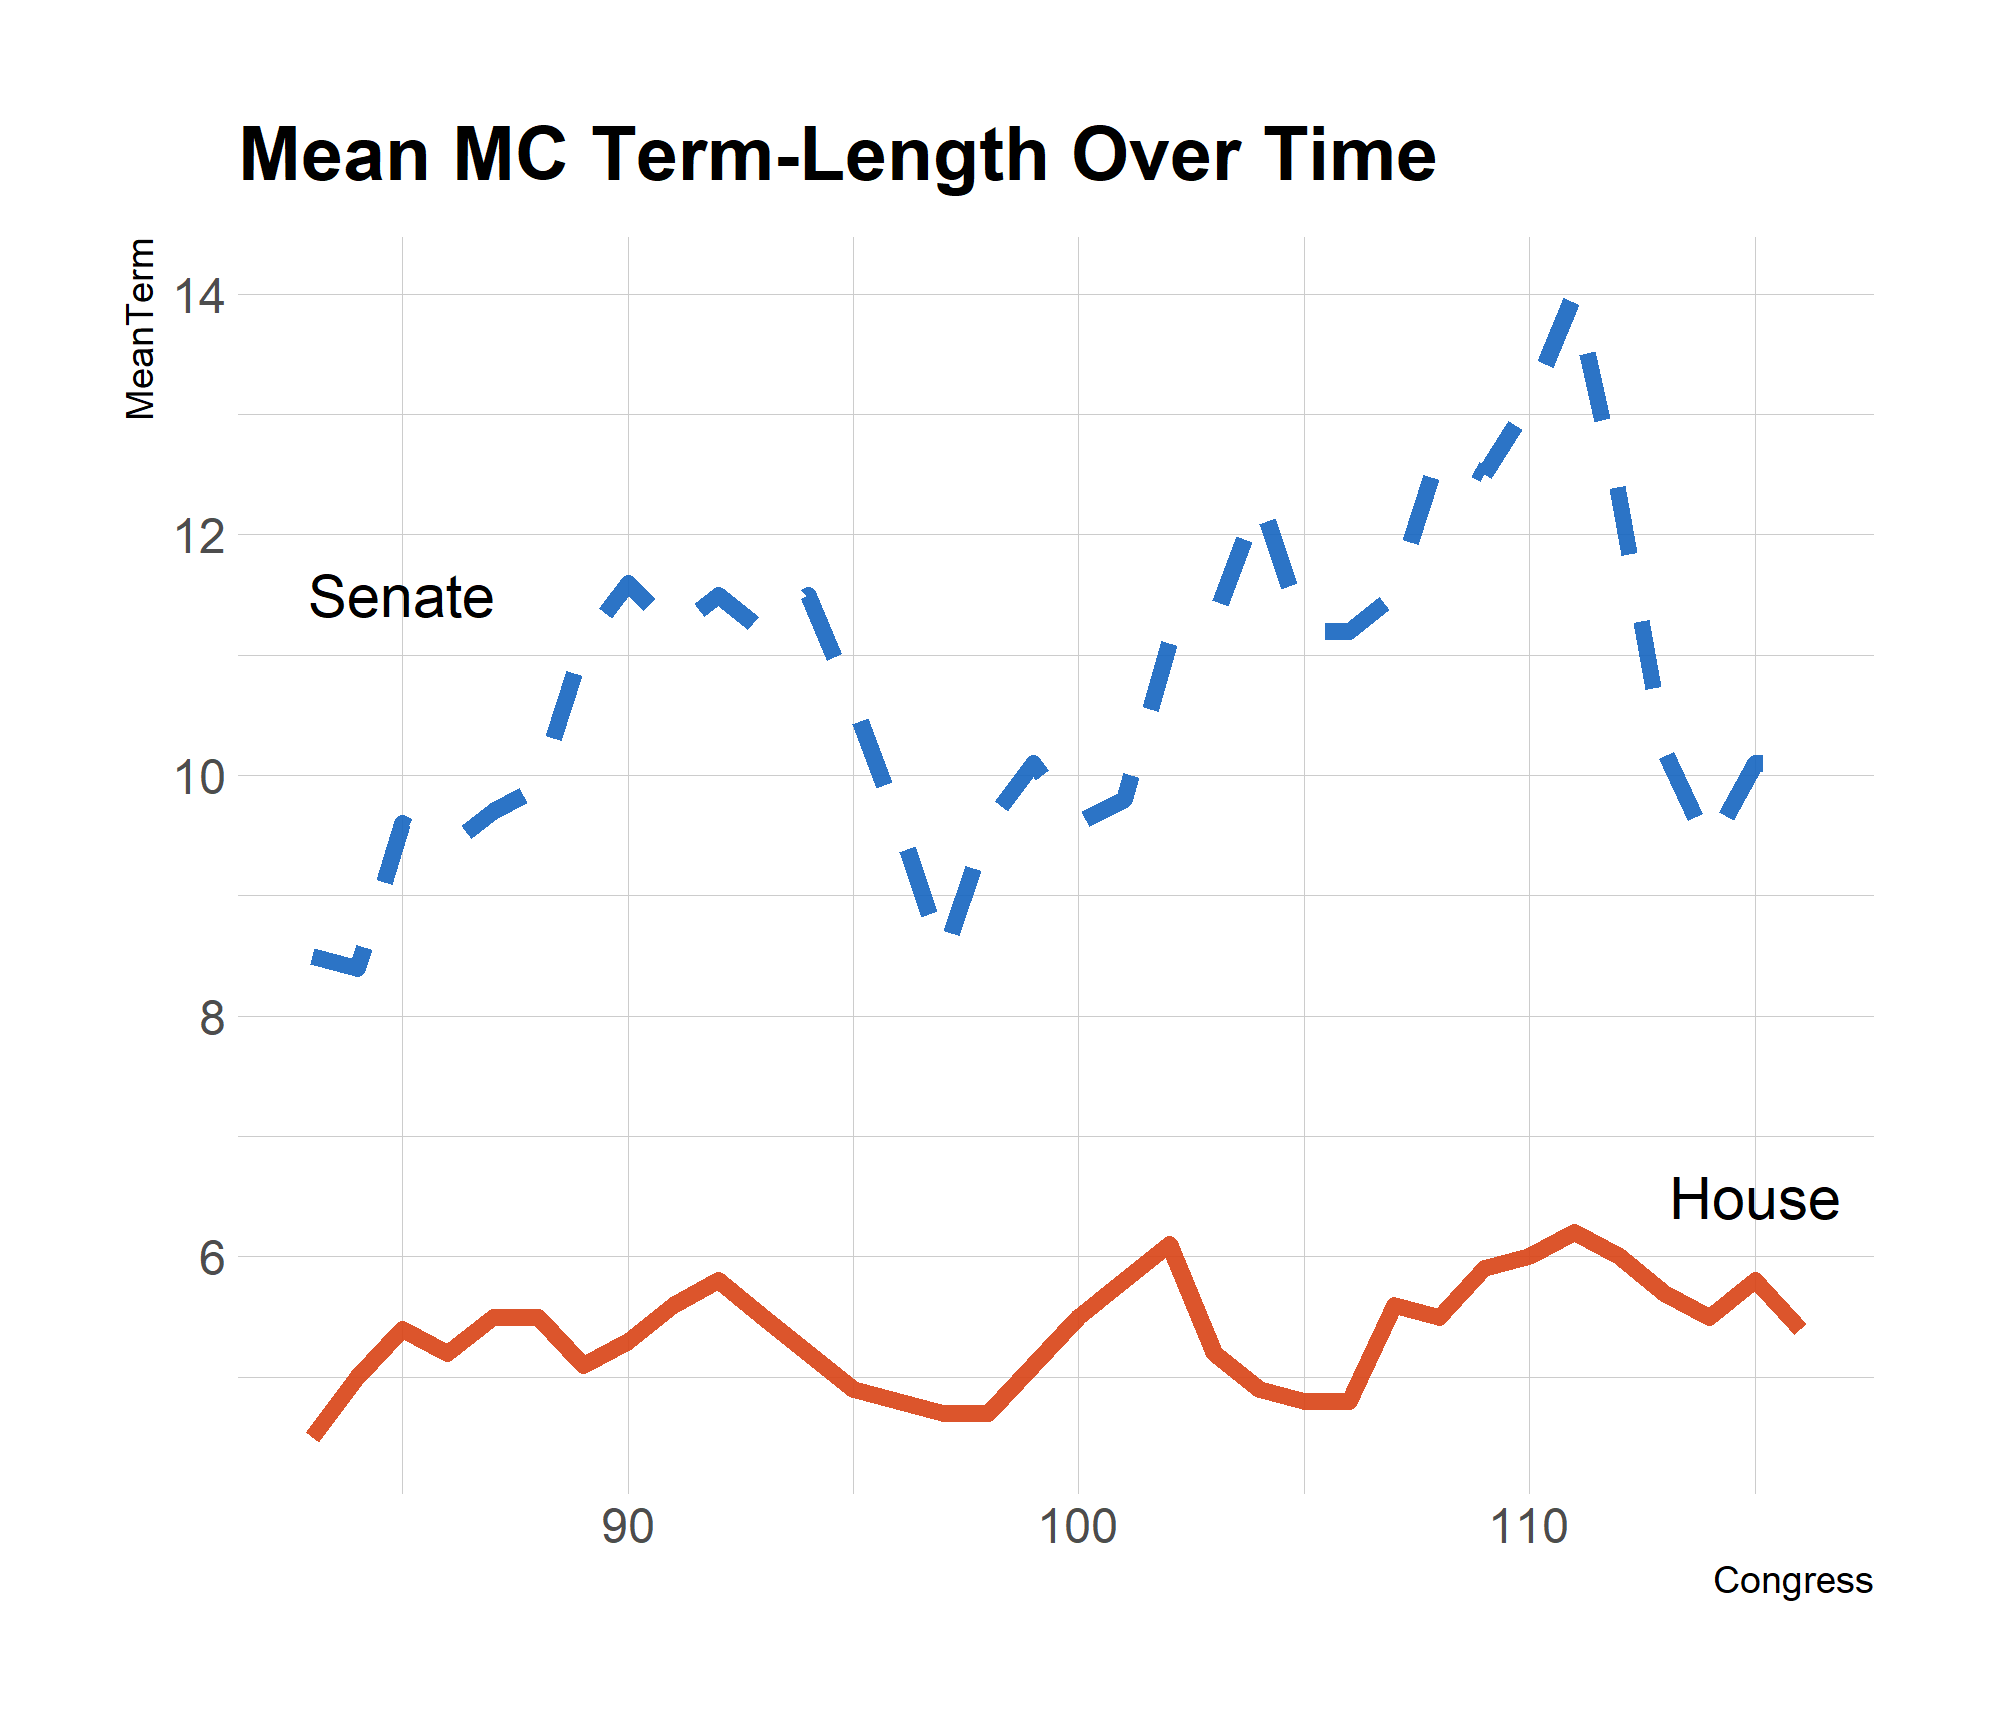
\includegraphics[height=300, width=400]{../figures/term-time-plot.png}

Here we see that in more recent sessions, overall, MC's are spending less time in office. Unsurprisingly, we see that Senator's are spending more time in Congress. Looking at the trend over time, it appears that for both chambers, the average number of terms an MC spends in office is increasing. Beyond the number of terms, the age of the average representative may be another important factor here. To elaborate on this point, age may be an important proxy for experience and expertise from prior careers and a proxy for professionalization. Age may also be an important control due to bias against youth in American politics. For example, It may be the case that a younger MC may be treated differently than an older but no-more senior colleague. 

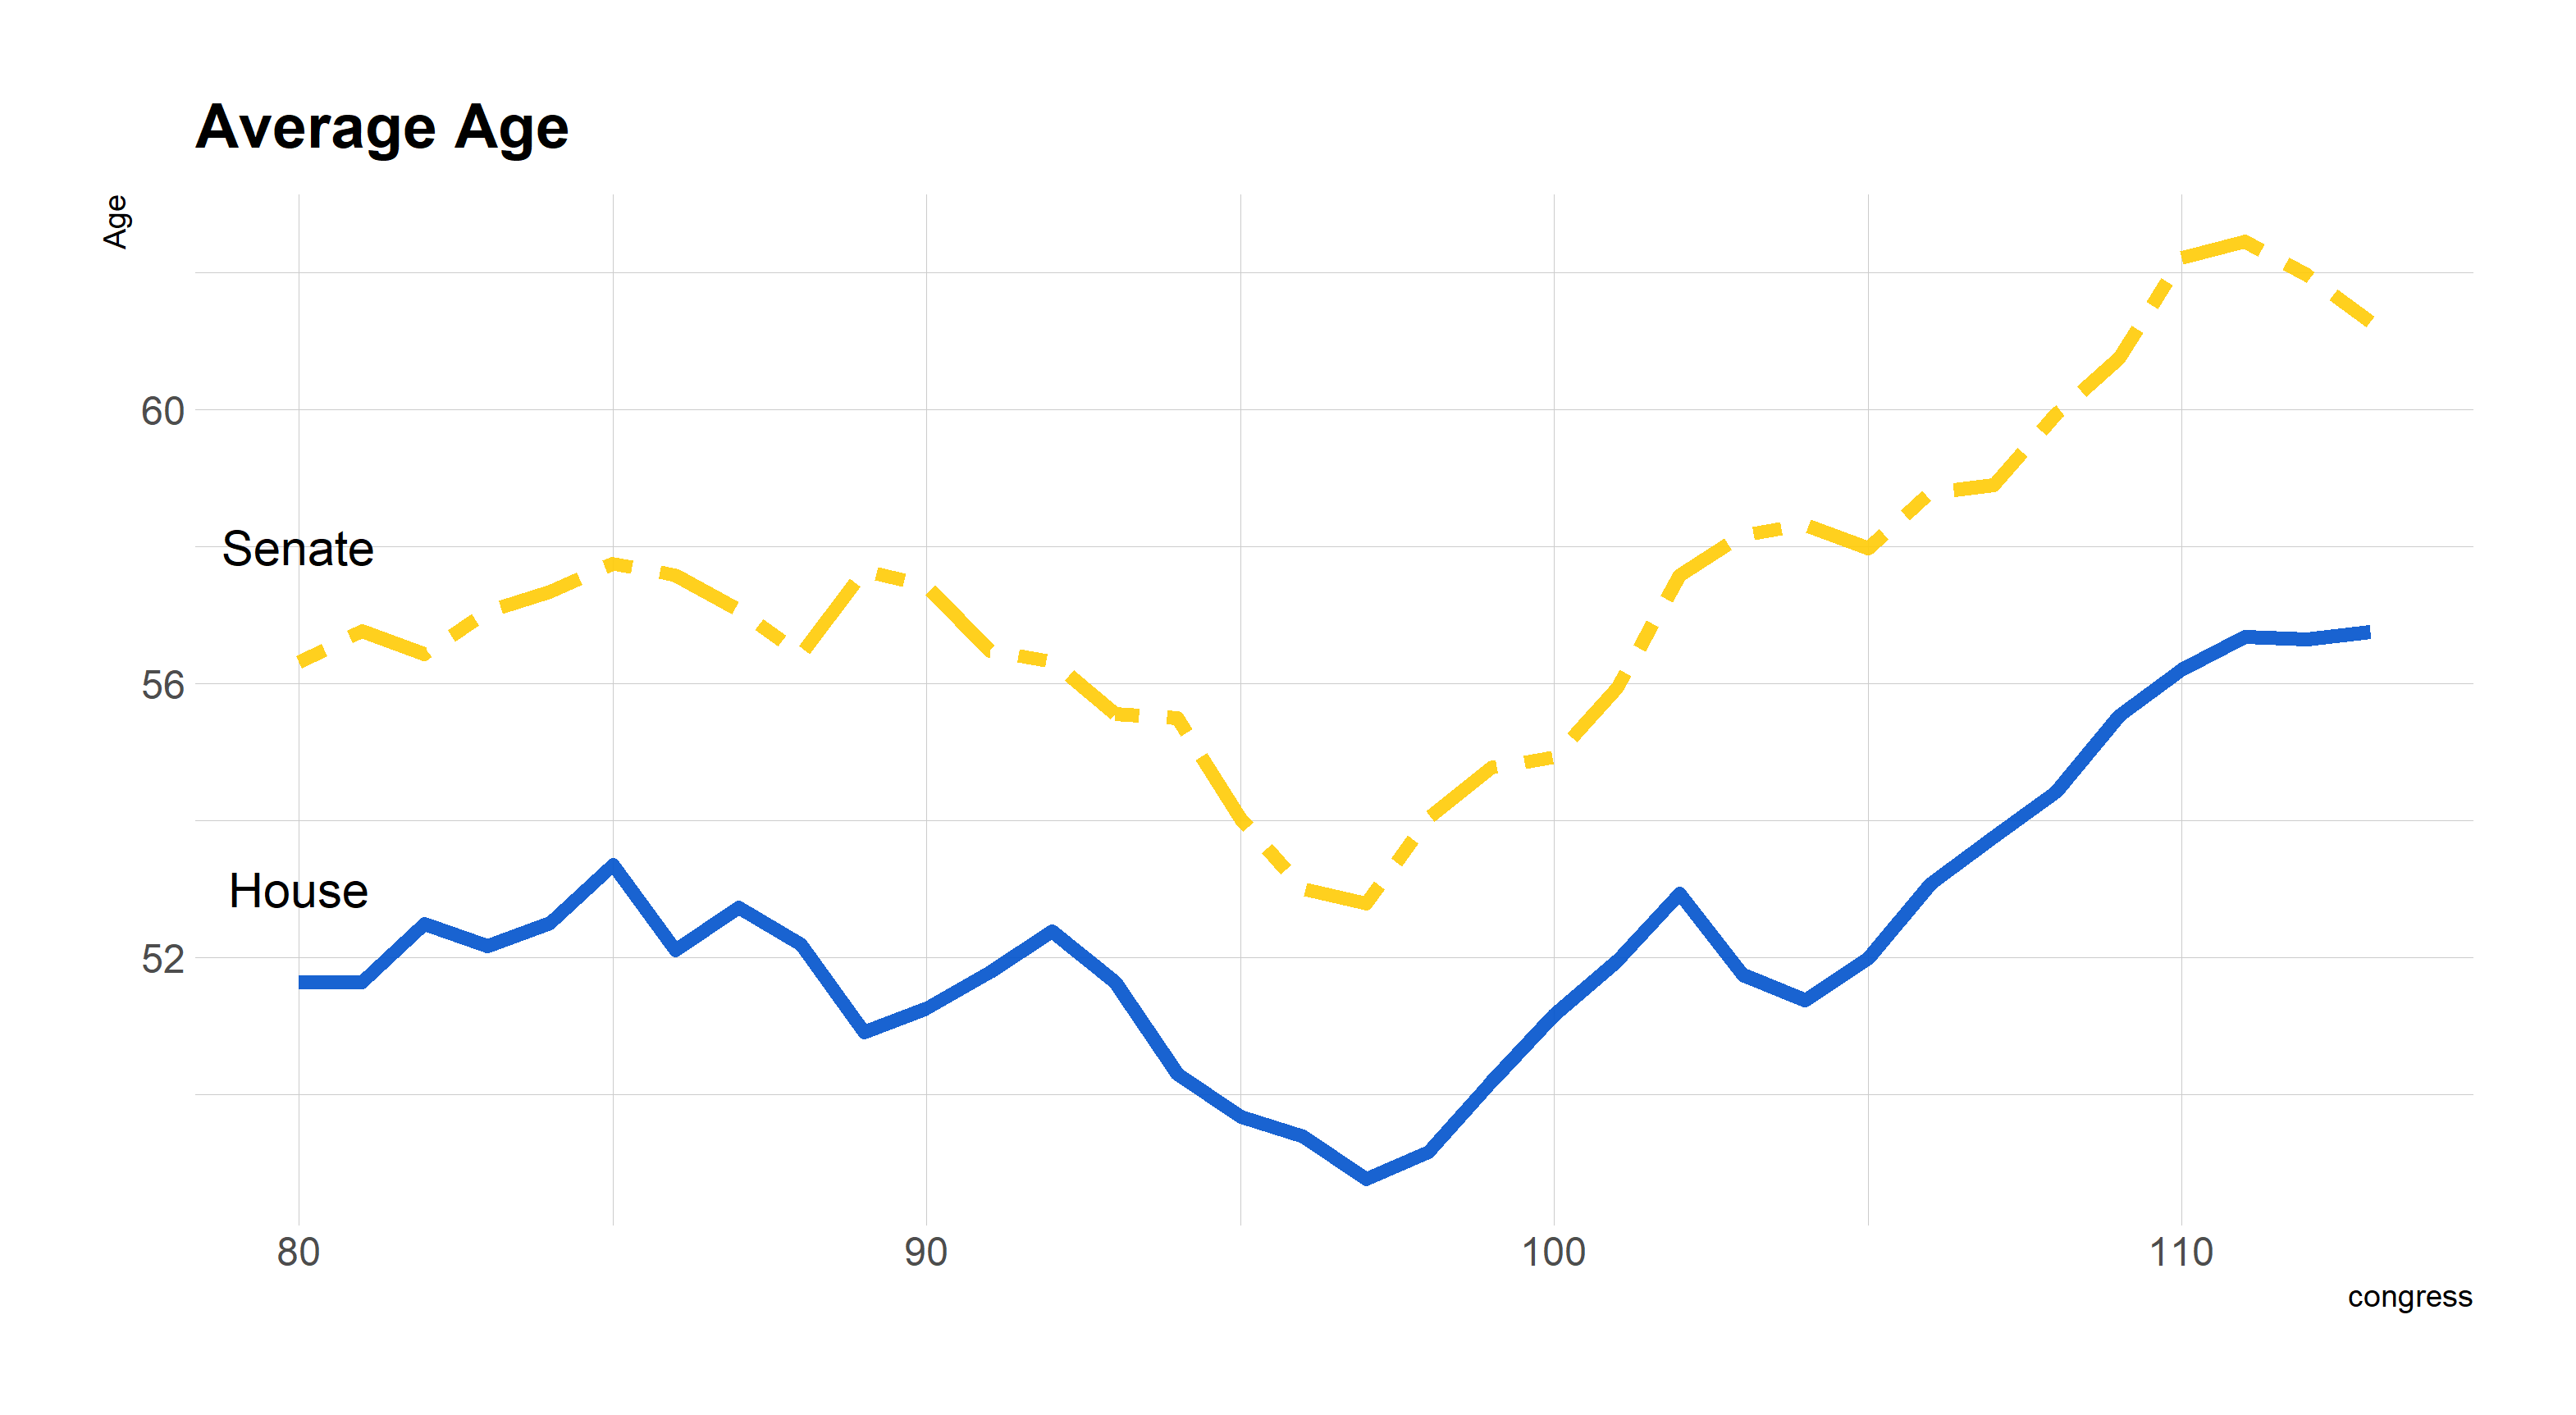
\includegraphics[height=300, width=400]{../figures/age-over-time}

The second figure presents data from FiveThirtyEight's Congress Age project. The data are the average of all MC's in each chamber for that given session. We see that over time, MC's have become older. There appears to be a small inflection point near the end of FiveThirtyEight's dataset demonstrating there was a session or two that have been a bit younger than the years directly previous to t.

These figures so far only demonstrate the demographics of the entire Congress and does not focus on the members holding leadership positions. To most explicitly determine whether those holding leadership positions have had fewer terms as compared to in the past, I use Volden and Wiseman's data on the U.S. House that runs from the 1970's until the 2018 Congress. With that data, I subset my dataset to only include those in leadership positions (subcommittee or committee Chairs, Majority or Minority Leadership - as defined by Volden and Wiseman, or whether they held an Appropriation's Committee seat) for that particular session of Congress. I then calculated how many years that member had been in Congress based on the first year of the session they took office and the first year of the current term. To be transparent, this is still a descriptive analysis and is not multivariate. I then subsetted the data to separate out Republicans and Democrats since Democrats tend to descriptively be younger. I also standardized the average seniority of the members that met my conditions by dividing those averages per congress by that same congresses average number of years served among all members. This means that I did not control for any factors nor did I conduct any tests or corrections for the stationarity of the data - this is not an empirical model and is not correlational. The third figure presents a plot of these data.

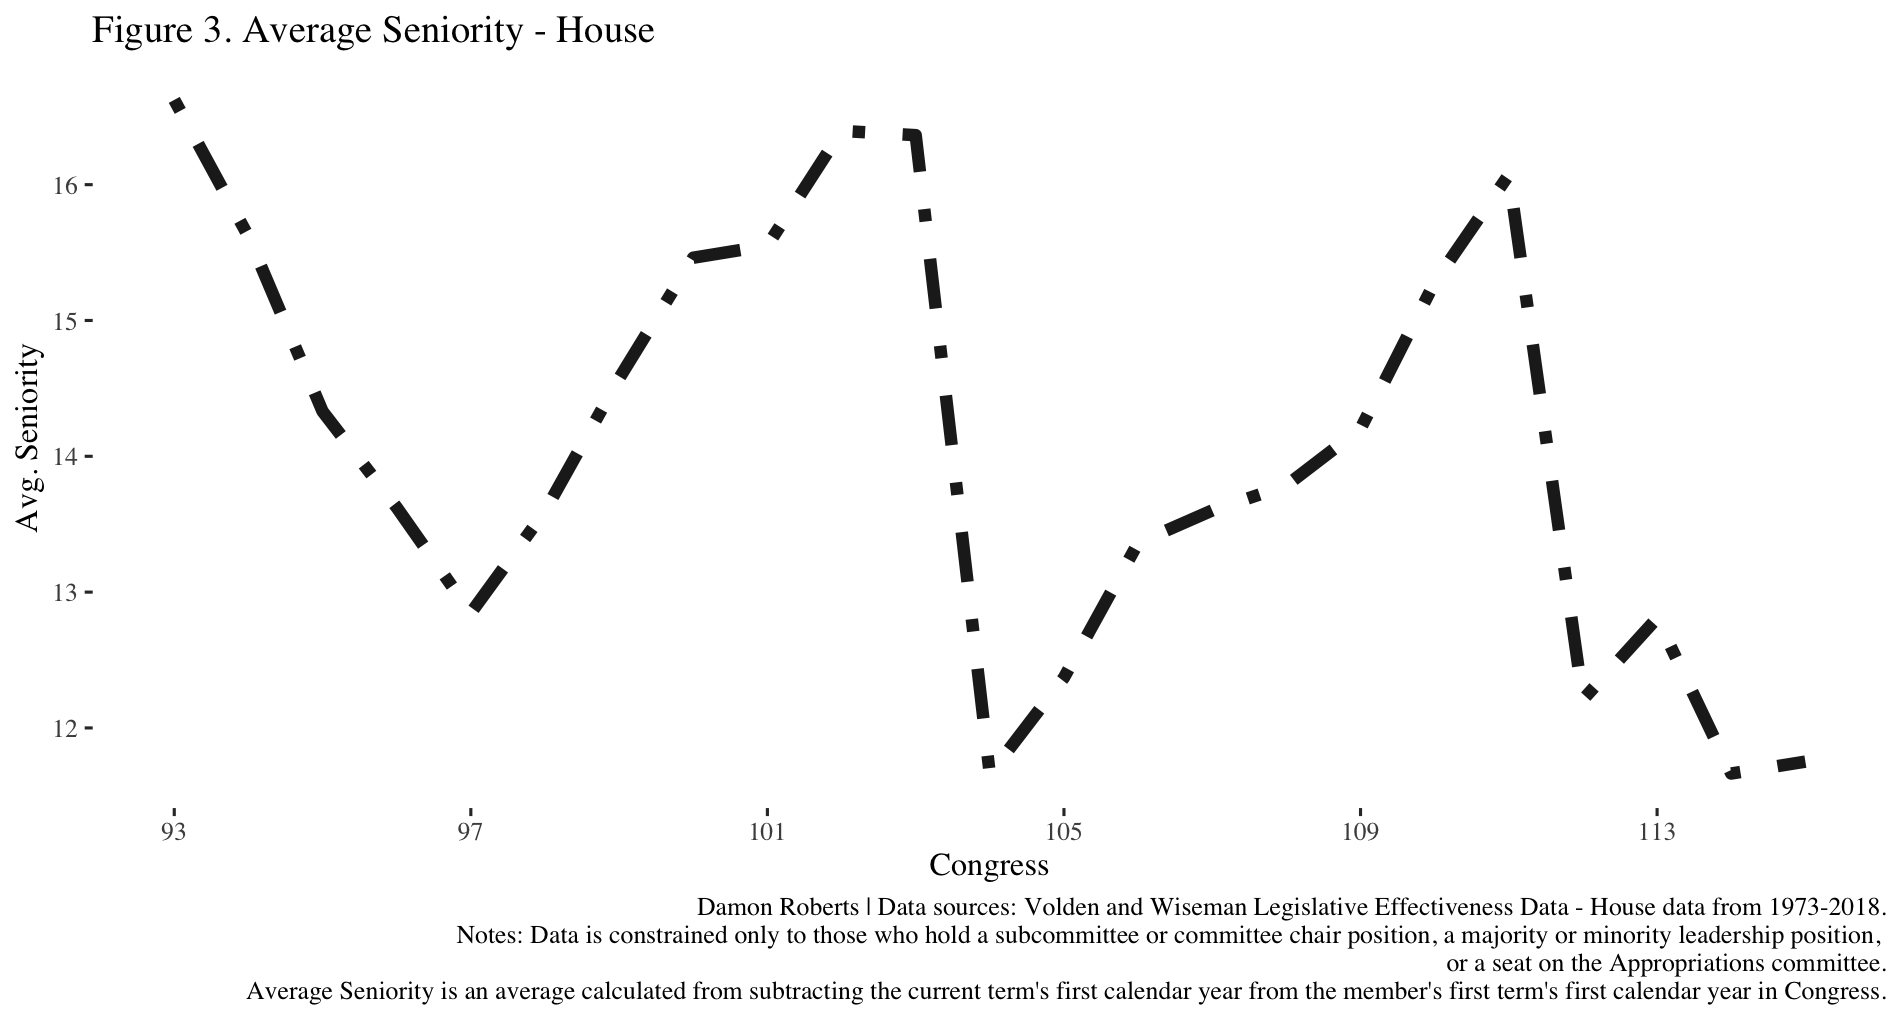
\includegraphics[height=400,width=400]{../figures/avg-house-seniority-macro.png}

These descriptive data demonstrate that there is a downward trend in holding any leadership position and the number of years on has been in office in the House of Representatives despite an increase in the number of terms for the average member of Congress. This graphic, while simple, provides some descriptive evidence that scholarly efforts to an increased attention of Congressional assignments are warranted. Specifically, it presents some basic evidence that there might not be a perfect correlation between seniority and leadership assignment and perhaps this correlation is decreasing over time as well. This figure also demonstrates that a claim of plausibly statistically significant alternative explanations besides seniority for leadership assignment in the House has empirical support. 

It is important here to not conflate the number of terms with seniority violations, however. To be sure to not overstate the takeaways a reader should have from the figure, it the differences between seniority and term length should be identified before moving on. When scholars operationalize seniority, they are referring to the length of time \textit{within} the committee or subcommittee and not overall length of time in the chamber. The figure presented here, presents time in the chamber and not within assignments. This is one of the key challenges with quantifying the seniority system - the need to identify violations of seniority within subcommittees and committees as opposed to using the more widely available data on the chambers as a whole. 

\section*{Discussion and Conclusion}

Observing that seniority has decreased in the House of Representatives since the 1970's among those holding leadership positions despite a much more stable trend of term length of the average member of Congress and an increasing age of the average member of Congress, this indicates a need for further scholarly exploration of the incentives a majority caucus may pursue as an alternative to within caucus seniority. 

In this paper, I argue that there are in fact a number of interesting alternative incentives and a resulting bargaining structure that guide the majority caucus' decisions for leadership assignments. Specifically, my theory posits that this is most likely to occur when there are relatively weaker - defined broadly as those who provide fewer benefits to the caucus - incumbents in leadership positions. From this, I add that this is increasing in a post-reform House where there is a higher barrier to entry from increasingly competitive House election races. The side effect of this is that higher commitments to your partisan teammates are quite an effective way to garner support for your leadership in the chamber.

This bargain implies a strong interdependence among copartisan colleagues for the realization of their career goals. This model also more centrally associates the informal seniority system with the motivations first discussed by \citeA{Fenno1973} and \citeA{Mayhew1974}. The model also demonstrates that the seniority system is quite a useful heuristic for the caucus and its leadership. In many situations, the status quo is a common outcome. Only situations where the incumbent is relatively weak and there are viable alternative options are an important factor for determining a deviation from the seniority system. 

Due to the complexity of this topic and phenomenon, there are certainly valuable areas for future research that this project, as it stands, has not addressed completely, or at all. Future iterations of this project, and possibly other projects, would benefit from a more thorough and complete discussion of the different types of incentives that parties and individuals may face as opposed to my model's focus on a more aggregative view of relative benefits that a particular sub-committee, committee, or caucus can gain from its members and current leaders. Relatedly, future iterations of the project should engage more with the clearly present tension between how the theory accounts for individual and collective motivations. In regards to developing the theory more, the paper future iterations should also more seriously engage with what the incentive structure looks like in a more dynamic world - this model is overly simplistic and focuses narrowly on only a few factors. The future iterations of this project and future work should also extend itself to collect data like Ponder and Renka's that not only descriptively demonstrates situations in which the caucus violates the seniority rule but also attaches it to relevant and significant demographic factors of individual MC's. This data would be tremendous in identifying the relative importance of different demographical and contextual motivations for the leadership and collective caucus to support a deviation from the seniority system. As polarization increases and as the perceived stakes of winning a majority in Congress heighten, understanding the electoral and alternate motives for supporting newer members also becomes more central to understanding the evolution of Congress.

\newpage
\bibliographystyle{apacite}
\bibliography{/Users/damonroberts/Dropbox/Bibliographies/Krehbiel1991,/Users/damonroberts/Dropbox/Bibliographies/Celler1961,/Users/damonroberts/Dropbox/Bibliographies/Mayhew1974,/Users/damonroberts/Dropbox/Bibliographies/Cox2005,/Users/damonroberts/Dropbox/Bibliographies/Rhode1991a,/Users/damonroberts/Dropbox/Bibliographies/Fenno1973,/Users/damonroberts/Dropbox/Bibliographies/Aldrich,/Users/damonroberts/Dropbox/Bibliographies/McKelvey1992,/Users/damonroberts/Dropbox/Bibliographies/Taylor2019,/Users/damonroberts/Dropbox/Bibliographies/Austen-Smith1993,/Users/damonroberts/Dropbox/Bibliographies/Hall2006,/Users/damonroberts/Dropbox/Bibliographies/McCrain2018,/Users/damonroberts/Dropbox/Bibliographies/Ansolabehere2014,/Users/damonroberts/Dropbox/Bibliographies/Utych2019,/Users/damonroberts/Dropbox/Bibliographies/Kellermann2009}
\end{document}